\section{Other platforms}
\label{sec-evaluation-other-platforms}



\begin{figure}
    \centering
    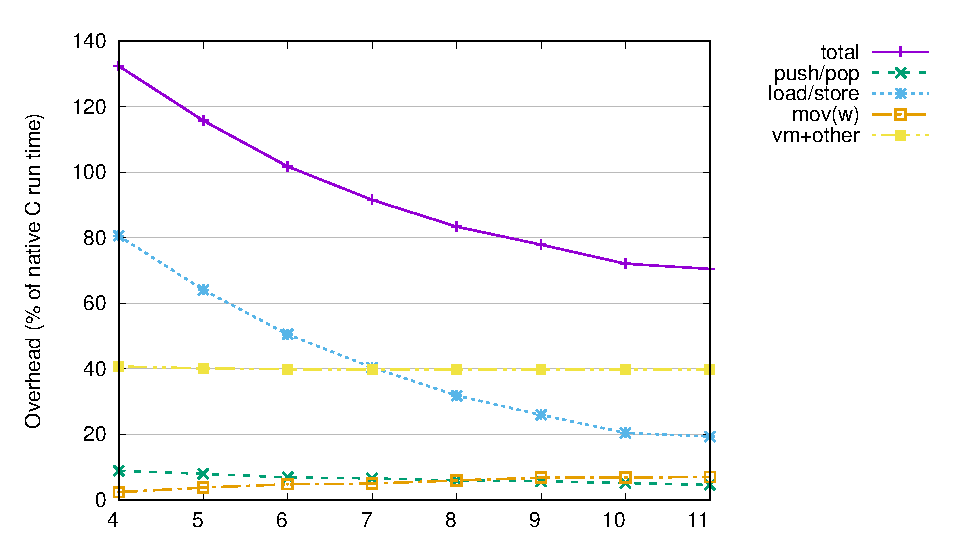
\includegraphics[width=\myfiguresizeperformance]{cachesize-performance-per-opcode-category.eps}
    \caption{Performance for different stack cache sizes (in pairs of registers)}
    \label{fig-performance-per-opcode-category-per-cachesize}
\end{figure}

\begin{figure}
    \centering
    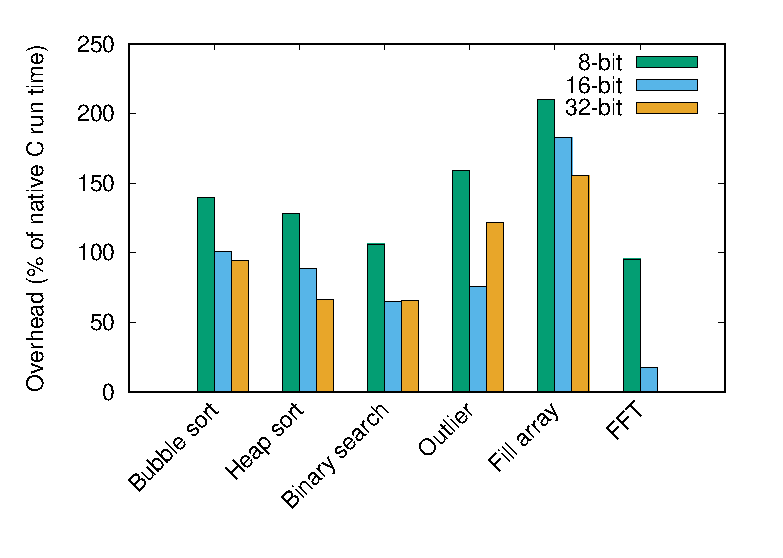
\includegraphics[width=\myfiguresizeperformance]{8_16_32_bit.eps}
    \caption{Performance for different data sizes}
    \label{fig-8_16_32_bit}
\end{figure}


\begin{table}
\caption{Performance overhead for different stack cache sizes (in pairs of registers)}
\label{tbl-performance-per-opcode-category-per-cachesize}
    \begin{tabular}{lrrrrrr} % UPDATED 20180327
    \toprule
    Number of                      & \multicolumn{5}{l}{Overhead} \\
    register pairs                 &  push/pop &   load/store &      mov(w) &    vm+other & \makebox[0.2mm]{}   &   total \\
    \midrule
    \midrule
      4                            &       8.7 &         80.5 &         2.4 &        38.1 &                     &   129.7 \\
      5                            &       7.8 &         64.0 &         3.8 &        37.5 &                     &   113.0 \\
      6                            &       6.7 &         50.3 &         4.7 &        37.0 &                     &    98.7 \\
      7                            &       6.4 &         40.2 &         4.9 &        37.0 &                     &    88.4 \\
      8                            &       5.7 &         31.6 &         5.8 &        36.9 &                     &    80.1 \\
      9                            &       5.5 &         25.6 &         6.7 &        36.9 &                     &    74.6 \\
     10                            &       4.9 &         20.1 &         6.8 &        36.9 &                     &    68.7 \\
     11                            &       4.3 &         18.9 &         6.9 &        36.9 &                     &    67.0 \\
    \bottomrule
    \end{tabular}
\end{table}

% UPDATED 20180214

\begin{table}[]
\centering
\caption{Performance for different data sizes}
\label{tbl-performance-8-16-32-bit}
\begin{tabular}{lrrr}
\toprule
               &   8-bit  &  16-bit  &     32-bit \\
\midrule
Bubble sort    &    139.5 &    101.2 &       94.4 \\
Heap sort      &    128.4 &     88.5 &       66.2 \\
Binary search  &    106.3 &     65.2 &         66 \\
Outlier        &      159 &     75.7 &      121.6 \\
FFT            &     96.7 &     17.7 &            \\
\bottomrule
\end{tabular}
\end{table}



%TODO explain why outlier32u is slower than 16: Mismatch between Proguard and the infuser. The infuser replaces integer opcodes with short versions where it can. ProGuard works on the original Java source and tries to reduce the number of variable slots by using the same slot for two variables if their live ranges do not overlap. In this case a short and int variable where mapped to the same slot which means to the infuser both now look like ints, so operations on the short variable, which is heavily used in the inner loop are now much more expensive. Again, this is another example where performance could be improved by combining the compiler, optimiser and infuser in a single optimising Java to MyVM bytecode compiler.